\chapter{Effects of alloying elements on the elastic properties of bcc ternary and higher ordered Ti-alloys}

\section{Introduction}

In order to develop a better understanding about alloying effect on the elastic properties of Ti alloys, the present work is developing an elastic database for the Ti-Mo-Nb-Sn-Ta-Zr system. With the focus being on bcc Ti-alloys, the effects of alloying elements on the pure elements and Ti-X binary alloys in the bcc phase were calculated in chapter 5. After extrapolating to higher order systems, it was hypothesized that studying the effects of alloying on the elastic properties of ternary alloys would improve the database. The present work focuses on studying the elastic properties of the Ti-X-Y (X $\neq$Y = Mo, Nb, Ta, Sn, and Zr) ternary alloys in the bcc phase. The single crystal elastic stiffness constants (cij’s) and polycrystalline aggregate properties are predicted across the composition range using Density Functional Theory (DFT) at 0 $^\circ$K outlined in the methodology chapter. Based on the DFT results, the CALPHAD approach outlined in the methodology is used to evaluate ternary interaction parameters. The interaction parameters are then incorporated into the database and the database accuracy is again tested similarily to the testing in chapter 5. The completed database is used to map the elastic modulus as a function of compostion. 

\section{Modeling and Calculations}

\subsection{Calculation details}

To study the elastic properties of the ternary bcc Ti alloys in the Ti-Mo-Nb-Sn-Ta-Zr system, first-principles calculations based on density functional theory were completed using the VASP (Vienna ab-initio simulation package) \cite{Kresse1996,Kresse1999}. Four calculations were done for each ternary alloy Ti-X-Y, with the varying compositions of X$_{0.5}$Y$_{0.5}$ (16-atom supercell), TiXY (36 atoms), Ti$_2$XY (32 atoms), Ti$_6$XY (64 atoms). The structures were all special quasirandom structures (SQS) that were previously generated by Jiang et al. \cite{Jiang2004,Jiang2009}. Due to instability of some of these structures in the bcc phase, different relaxation schemes were used to retain the strucutral symmetry while obtaining the lowest energy structure. These relaxation schemes are outlined in the methodology chapter under the SQS section. The projector augmented wave (PAW) method was used to describe the ion-electron interaction. Based on the work of comparing X-C functionals (Figure \ref{Ch2-figure:PBEvsPW91}) the exchange-correlation functional of the generalized gradient approach depicted by Perdew, Burke, and Ernzerhof (PBE) was employed \cite{Perdew1996a}. An energy cutoff roughly 1.3 times higher than the default value, 310, was used for all calculations. The valance configuration for each element was selected based on the VASP recommendations and is listed in the methodology chapter. The Brillouin zone sampling is done using the gamma centered Monkhorst-Pack scheme \cite{Monkhorst1976a}. The elastic calculations were completed using a strain magnitude of $\pm$0.01 based on the study done in chapter 5 and the results seen in Figure \ref{Ch5-figure:Strain}.

\subsection{Modeling details}

The first-principles results are then used to model the elastic stiffness constants. The modeling was completed by plotting the binary interpolation from the working database build in chapter 5. The plots started at X$_{0.5}$Y$_{0.5}$ and plotted ot pure Ti. The difference between the binary interpolation and the first-principles results were calculated. The differences were then used to obtain a single fitting parameter using the mathematica code in appendix c. With the focus being Ti-rich alloys and wanting to follow the same modeling technique used on the binary alloys, the first-principles results with 70 at.\% Ti or higher were weighted heavier (x6, according to the authors' practices) than the other points for the fittings. The best fit was found and the ternary interaction parameters were incorporated into the database. The databases was then used to predict the moduli values of the ternary alloys. 

\section{Results and discussion}

\subsection{Elastic calculation results}

The calculated elastic stiffness constants and moduli values are listed in Table \ref{Ch6-table:tixyelasdata} with the experimental values used for comparison. Figure \ref{Ch6-figure:tixyyoungs1} and \ref{Ch6-figure:tixyyoungs2} plot the Young's modulus calculations (circles) for each Ti-X-Y ternary system (X$\neq$Y= Mo, Nb, Sn, Ta, Zr) starting from a 50-50 mixture of the two alloying elements to Ti. The red dashed line is an interpolation from the binary interaction parameters shown in Table \ref{Ch5-table:tixelasip}. The Voigt high bound is plotted as a purple dotted line with the Reuss low bound plotted as a gold dotted-dashed line and the Hill average is plotted as a solid black line. The Voigt and Reuss bounds vary more drastically when the bcc structure is unstable as opposed to when the bcc structure is stable. The database predicts the Hill average.  When possible \textit{E} data obtained experimentally is plotted for comparison. 

The present \textit{E} results for the Ti-Mo-Nb (Figure \ref{Ch6-figure:tixyyoungs1}a) alloy system are compared with \textit{E} data from Niinomi et al. \cite{Niinomi2012} obtained experimentally. The error between the previous results and present results was calculated using Eq. Y. The \textit{E} results from Niinomi et al. are closer to the Voigt bound than Hill average and has an error of 0.65. The present data shows that the \textit{E} decreases from Mo0.5Nb0.5 to Ti. From the literature search, no bcc Ti-Mo-Sn (Figure \ref{Ch6-figure:tixyyoungs1}b) experimental \textit{E} results were available to compare with the present work. The \textit{E} trend shows a decrease in value from Mo$_{0.5}$Sn$_{0.5}$ to Ti.  The calculated \textit{E} results for the Ti-Mo-Ta alloy system (Figure \ref{Ch6-figure:tixyyoungs1}c) are compared with experimental data from Niinomi et al. \cite{Niinomi2012} and Mohammad et al. \cite{Mohammed2014} showing an error of 0.46 (Eq. Y). The \textit{E} values from Niinomi et al. and Mohammad fit well with the present Voigt bound. The \textit{E} data decreases in value from Mo$_{0.5}$Ta$_{0.5}$ to Ti. The Young's modulus of the Ti-Mo-Zr alloy system (Figure \ref{Ch6-figure:tixyyoungs1}d) is compared with experimental \textit{E} values from Mohammad et al. \cite{Mohammed2014}. The experimental \textit{E} from Mohammad et al. and the present \textit{E} vary by less than 6 GPa and shows the Young's modulus values decreases from Mo$_{0.5}$Zr$_{0.5}$ to Ti. Experimental \textit{E} results from Niinomi et al. \cite{Niinomi2012}, Mohammad et al. \cite{Mohammed2014}, and Nozoe et al. \cite{Nozoe2007} are compared with the present \textit{E} calculations for the Ti-Nb-Sn alloy system (Figure \ref{Ch6-figure:tixyyoungs1}e). The experimental \textit{E} results from Niinomi et al, Mohammad et al. and Nozoe et al. fit within the present Voigt-Reuss bounds and have an error of 0.39 from the present Hill average \textit{E} values. The data trend in the \textit{E} values shows an increase in the \textit{E} value from Nb$_{0.5}$Sn$_{0.5}$ to 50 at \% Ti and then a decrease in value to Ti.   

Figure \ref{Ch6-figure:tixyyoungs2} continues to plot the \textit{E} of the Ti-X-Y ternary alloy systems. Figure \ref{Ch6-figure:tixyyoungs2}a, plots the present \textit{E} results for the Ti-Nb-Ta alloy system, versus the \textit{E} results from Mohammad et al. \cite{Mohammed2014}. The \textit{E} results from Mohammad et al. fit along the Reuss bound and using Eq. Y have an error of 0.28 from the present \textit{E} values. The Young's modulus decreses from Nb$_{0.5}$Ta$_{0.5}$ to Ti. The present \textit{E} for the Ti-Nb-Zr (Figure \ref{Ch6-figure:tixyyoungs2}b) alloy system is compared with \textit{E} results obtained experimentally by Geetha et al. \cite{Geetha2009},  Mohammad et al. \cite{Mohammed2014}, and Niinomi et al. \cite{Niinomi2012}. The \textit{E} results from Geetha, Mohammad and Niinomi fit well between the Voigt-Reuss bounds and have an error of 0.08 from the present Hill average \textit{E} results. The \textit{E} shows an increase in value from Nb$_{0.5}$Zr$_{0.5}$ to 70 at \% Ti and then a decrease to Ti. The Ti-Sn-Ta, Ti-Sn-Zr and Ti-Ta-Zr alloy systems are not compared with any experimental data in Figure \ref{Ch6-figure:tixyyoungs2}c, d and e respectively. The trend in the \textit{E} data for the Ti-Sn-Ta alloy system shows that the \textit{E} decreases from Sn$_{0.5}$Ta$_{0.5}$ to Ti. The Ti-Sn-Zr alloy system data shows an increase in the \textit{E} values from Sn$_{0.5}$Zr$_{0.5}$ to 60 at \% Ti and then the \textit{E} decreases to Ti. The \textit{E} values, for the Ti-Ta-Zr alloy system, show the \textit{E} decreases to 15 at \% Ti where the \textit{E} begins increasing to 30 at \% Ti and then decreases to Ti. 

The error between the experimentally determined \textit{E} and the present first-principles calculated \textit{E} results is expected to occur due to the fact that the CALPHAD fittings are done using elastic stiffness constants calculations done at 0 $^\circ$K on single crystal structures while the experiments are done measuring polycrystalline samples at 300 $^\circ$K. While there is some error, the experiments fit well within the bounds set by Reuss and Voigt and the Hill average generally reproduces the experimentally determined \textit{E} data for the Ti-X-Y ternary alloys. 

The elastic stiffness constants, $\overline{C}_{11}$, $\overline{C}_{12}$, and $\overline{C}_{44}$ are plotted in Figure \ref{Ch6-figure:tixyc11_1} to Figure \ref{Ch6-figure:tixyc44_2}. The $\overline{C}_{11}$ data showed similar trends for most of the Ti-X-Y systems where the $\overline{C}_{11}$ values decrease from X$_{0.5}$Y$_{0.5}$ to Ti (seen in Figure \ref{Ch6-figure:tixyc11_1} and Figure \ref{Ch6-figure:tixyc11_2}). The  data trends vary for the Ti-Sn-Zr and Ti-Ta-Zr alloy systems in Figure \ref{Ch6-figure:tixyc11_2}d and e, respectively. The $\overline{C}_{11}$ values, for Ti-Sn-Zr system, increases to 60 at \% Ti and then decreases to Ti, while the $\overline{C}_{11}$ values, in the Ti-Ta-Zr system, increase to 35 at \% Ti and then decreases to Ti. 

The  $\overline{C}_{12}$ values plotted in Figure \ref{Ch6-figure:tixyc12_1} and \ref{Ch6-figure:tixyc12_2}, decrease from X$_{0.5}$Y$_{0.5}$ to Ti similarly for the Ti-Mo-Nb, Ti-Mo-Ta and Ti-Nb-Ta systems. The Ti-Mo-Sn and Ti-Nb-Sn systems saw a decrease in $\overline{C}_{12}$ value from X$_{0.5}$Y$_{0.5}$ to 15 at \% Ti then and increase to 85 \% Ti and then a decrease to Ti. The Ti-Mo-Zr and Ti-Nb-Zr systems show a decrease in $\overline{C}_{12}$ value from X$_{0.5}$Y$_{0.5}$ to 60 at \% Ti and then an increase to Ti. The $\overline{C}_{12}$ values increase from X$_{0.5}$Y$_{0.5}$ to 70 at \% Ti and then decrease to Ti for the Ti-Sn-Ta system. For the Ti-Sn-Zr system, the $\overline{C}_{12}$ values increase from X$_{0.5}$Y$_{0.5}$ to Ti and the $\overline{C}_{12}$ values, for the Ti-Ta-Zr system, decrease to 70 at \% Ti and then increase. 

The $\overline{C}_{44}$ data plotted in Figure \ref{Ch6-figure:tixyc44_1} and Figure \ref{Ch6-figure:tixyc44_2} shows that the values similarly decrease from X$_{0.5}$Y$_{0.5}$ to Ti for the Ti-Mo-Sn and Ti-Ta-Zr systems. The Ti-Mo-Zr and Ti-Mo-Ta systems show that the $\overline{C}_{44}$ values decrease from X$_{0.5}$Y$_{0.5}$ to 80 at \% Ti and then increase to Ti. The $\overline{C}_{44}$ values, for the Ti-Mo-Nb and Ti-Nb-Ta systems, show a decrease from X$_{0.5}$Y$_{0.5}$ to 65 at \% Ti and then increasing to Ti. The $\overline{C}_{44}$ values show an increase from X$_{0.5}$Y$_{0.5}$ to 80 at \% Ti and then a decrease to Ti for the Ti-Nb-Sn and Ti-Nb-Zr systems. The $\overline{C}_{44}$ values, for the Ti-Sn-Ta system, decrease from X$_{0.5}$Y$_{0.5}$ until 20 at \% Ti, then increase to 50 at \% Ti and then decrease to Ti. Finally the Ti-Sn-Zr system shows an increase in $\overline{C}_{44}$ value from X$_{0.5}$Y$_{0.5}$ to 60 at \% Ti and then decrease to Ti. 

The $\overline{C}_{11}-\overline{C}_{12}$ is plotted in Figure \ref{Ch6-figure:tixyc11-c12}. The $\overline{C}_{11}-\overline{C}_{12}$ plot shows the limit of mechanical stability of the bcc phase for each ternary alloy. Based on Born’s criteria when the $\overline{C}_{11}-\overline{C}_{12}$ values are negative then the phase, bcc in this case, loses mechanical stability. Based on the present results in Figure \ref{Ch6-figure:tixyc11-c12}, the bcc phase loses mechanical stability in Ti-Mo-Nb, Ti-Mo-Ta, Ti-Mo-Zr, Ti-Nb-Zr, Ti-Sn-Zr, and Ti-Ta-Zr systems when the Ti concentration is more than 90 at \%, with the values being 91, 92, 95, 93, 91, and 94 at \% Ti respectively. The bcc phase loses mechanical stability at Ti concentrations of 87, 77, 89, and 80 at \% Ti for Ti-Mo-Sn, Ti-Nb-Sn, Ti-Nb-Ta and Ti-Sn-Ta systems. The \textit{B} and \textit{G} moduli data are plotted similarly to the Young's modulus in Figure \ref{Ch6-figure:tixybulk1} to Figure \ref{Ch6-figure:tixyshear2}. The present \textit{B} and \textit{G} calculations (circles) are plotted with at interpolation from the binary interaction parameters (red dashed line), the Voigt (purple dotted line) and Reuss (gold dash-dotted line) bounds and the Hill average (solid black line). The \textit{B} data showed the same trend, decreasing in value from X$_{0.5}$Y$_{0.5}$ to Ti, for all the Ti-X-Y ternaries except Ti-Nb-Sn, Ti-Sn-Ta and Ti-Sn-Zr seen in Figure \ref{Ch6-figure:tixybulk1} and Figure \ref{Ch6-figure:tixybulk2}. The \textit{B} data for the Ti-Nb-Sn and Ti-Sn-Ta systems, decrease in value from X$_{0.5}$Y$_{0.5}$ to 10 at \% Ti and then increase to 55 at \% Ti and then decrease to Ti. The \textit{B} values, in the Ti-Sn-Zr alloy system, showed an increase in value from X$_{0.5}$Y$_{0.5}$ to 85 at \% Ti and then a decrease to Ti. The \textit{G} decrease in value from X$_{0.5}$Y$_{0.5}$ to Ti for all the ternary systems except Ti-Nb-Sn, Ti-Nb-Zr, Ti-Sn-Zr and Ti-Ta-Zr (Figure \ref{Ch6-figure:tixyshear1} and Figure \ref{Ch6-figure:tixyshear2}). The \textit{G} values increase from X$_{0.5}$Y$_{0.5}$ to 60 at \% Ti and then decrease to Ti for the Ti-Nb-Sn, Ti-Nb-Zr systems. The \textit{G} data for the Ti-Sn-Zr system increases in value and the \textit{G} decreases in value from X$_{0.5}$Y$_{0.5}$ to 5 at \% Ti and then increases to 35 at \% Ti before decreasing to Ti for the Ti-Ta-Zr system.

\subsection{Extrapolation to higher ordered systems}

Using the completed database and interaction parameters in Table \ref{Ch5-table:tixelasip} and Table \ref{Ch6-table:tixyelasip}, the elastic stiffness constants can be predicted and then the moduli values can be calculated and mapped. Figure \ref{Ch6-figure:tixymap1} and Figure \ref{Ch6-figure:tixymap2} uses the global minimization tools in pycalphad \cite{Otis2017} to map the Young's modulus based on composition for Ti-X-Y ternaries. The mapping can thus allow for regions with specific moduli values to be targeted.

The Young's modulus is predicted and compared with experimental results for higher order Ti alloys and the results are shown in Table \ref{Ch6-table:tixydatacomp} and Figure \ref{Ch6-figure:tixydatabase}. The same comparison was made in chapter 5 but using only the pure elements and binary interaction parameters. As in Chapter 5, Figure \ref{Ch6-figure:tixydatabase} plots the calculated \textit{E} versus the experimentally determined \textit{E} \cite{Mohammed2014,Geetha2009,Tane2010a}. The black diagonal line would be a perfect correlation between the predictions and experiments. The grey region is the average variance in the first-principles calculations when calculating the average elastic stiffness constants using Eq. Y-Eq. Y. The same higher order alloys were picked to compare the effect that introducing the ternary interaction parameters had. As discussed previously, the error bars plotted for the experiments come from the variance that was seen when comparing the experimentally determined \textit{E} at the same composition from Niinomi et al. \cite{Niinomi2012}, Geetha et al. \cite{Geetha2009}, Tane et al. \cite{Tane2010a}, and Mohammad et al. \cite{Mohammed2014}. The horizontal error bars are the Voigt and Reuss bounds. Previously, with no ternary interaction parameters the predictions and experimental results varied anywhere between 0.69 and 14 GPa and on average by 7 GPa. This was attributed to the fact that the single crystal elastic stiffness constants that are fit to obtain the moduli values were at 0 $^\circ$K while the experiments on the polycrystalline samples are at done at 300 $^\circ$K. It was predicted that introducing non-Ti containing binary interaction parameters and ternary interaction parameters would improve the database. The introduction of the ternary interaction parameters improved the predictions to vary anywhere from 0.39 to 13 GPa from the experimental values with an average variance of only 5 GPa. Thus the introduction of Ti-containing ternary interaction parameters improved the predictions and the database can accurately predict the Young's modulus of higher order Ti alloys.


\section{Conclusion}

The present work systematically calculates the elastic properties of the bcc Ti ternary alloys, including the elastic stiffness constants, bulk modulus, shear modulus, and Young's modulus. Six alloying elements, Mo, Nb, Sn, Ta and Zr were studied. The CALPHAD method was used to fit ternary interaction parameters. The fittings were done by calculating the difference between the first-principles calculations and the binary interpolations from the pure elements and binary interaction parameters previously determined. The differences were then used to determine the ternary interaction parameters. The present calculations showed that the bcc phase was mechanically stabilized at compositions less than 91, 92, 95, 93, 91, 94, 87, 77, 89, and 80 at \% Ti for the Ti-Mo-Nb, Ti-Mo-Ta, Ti-Mo-Zr, Ti-Nb-Zr, Ti-Sn-Zr, Ti-Ta-Zr, Ti-Mo-Sn, Ti-Nb-St, Ti-Nb-Ta and Ti-Sn-Ta alloys respectively. 

The Ti-Mo-Nb, Ti-Mo-Ta, Ti-Mo-Zr, and Ti-Nb-Ta alloys saw similar fitting trends. The ternary interaction parameters were combined with the previously determined pure elements and binary interaction parameters into one complete tdb database. The fittings were used to map some of the possible alloy compositions to find potential materials with a Young's modulus in the target range for biomedical load bearing implants. Overall, the introduction of the ternary interaction parameters improved the database’s ability to predict the Young's modulus of higher ordered alloys and the database is able to accurately predict the Young's modulus of Ti-alloys. It is hypothesized that the introduction of non-Ti containing interaction parameters would improve the database even further. The tdb file is attached in appendix d. 


\newpage
\begin{longtable}[H]{ c c c c c c c c}
	\caption{First-principles calculations of the elastic stiffness constants, bulk modulus \textit{B}, shear modulus \textit{G}, and Young's modulus \textit{E} in GPa for different atomic percent compositions of the bcc Ti-X-Y ternary systems at 0 $^\circ$K. As well as experimental data obtained for the Young's modulus at 300 $^\circ$K by the reference stated.} 	\label{Ch6-table:tixyelasdata} \\
	\hline
	Reference & Ti$_{1-2b}$X$_b$Y$_b$ & $\overline{C}_{11}$ & $\overline{C}_{11}$ & $\overline{C}_{11}$ & \textit{B} & \textit{G} & \textit{E}\\
	\hline
	\endhead
	\hline
	\endfoot
	This work & Ti & 93 & 115 & 41 & 108 & -12.91 & -40.34\\
	This work & TiMo$_{12.5}$Nb$_{12.5}$ & 155 & 121 $\pm$4 & 34 $\pm$4 & 132 $\pm$4 & 26 $\pm$4 & 73 $\pm$4\\
	This work & TiMo$_{25.0}$Nb$_{25.0}$ & 222 $\pm$3 & 129 $\pm$3 & 33 $\pm$3 & 160 $\pm$3 & 38 $\pm$3 & 105 $\pm$3\\
	This work & TiMo$_{33.3}$Nb$_{33.3}$ & 269 $\pm$5 & 134 $\pm$3 & 42 $\pm$4 & 179 $\pm$5 & 51 $\pm$5 & 139 $\pm$5\\
	This work & Mo$_{50}$Nb$_{50}$ & 414 $\pm$6 & 165 $\pm$3 & 68 & 248 $\pm$6 & 87 $\pm$6 & 233 $\pm$6\\
	Expt 300 K \cite{Niinomi2012} & TiMo$_{6}$Nb$_{2}$ & & & & & & 110\\
	This work & TiMo$_{12.5}$Sn$_{12.5}$ & 137 $\pm$15 & 121 $\pm$2 & 56 $\pm$13 & 126 $\pm$15 & 27 $\pm$15 & 75 +$\pm$15\\
	This work & TiMo$_{25.0}$Sn$_{25.0}$ & 160 $\pm$3 & 130 $\pm$8 & 71 $\pm$2 & 140 $\pm$8 & 39 $\pm$8 & 106 $\pm$8\\
	This work & TiMo$_{33.3}$Sn$_{33.3}$ & 167 $\pm$8 & 133 $\pm$6 & 75 $\pm$2 & 144 $\pm$8 & 42 $\pm$8 & 114 $\pm$8\\
	This work & Mo$_{50}$Sn$_{50}$ & 192 $\pm$28 & 130 $\pm$36 & 40 $\pm$31 & 151 $\pm$36 & 36 $\pm$36 & 100 $\pm$36\\
	This work & TiMo$_{12.5}$Ta$_{12.5}$ & 153 $\pm$1 & 125 $\pm$4 & 38 $\pm$3 & 134 $\pm$4 & 25 $\pm$4 & 72 $\pm$4\\
	This work & TiMo$_{25.0}$Ta$_{25.0}$ & 222 $\pm$2 & 136 $\pm$1 & 45 $\pm$3 & 165 $\pm$2 & 44 $\pm$3 & 122 $\pm$3\\
	This work & TiMo$_{33.3}$Ta$_{33.3}$ & 263 $\pm$4 & 145 $\pm$6 & 49 $\pm$4 & 184 $\pm$6 & 53 $\pm$6 & 145 $\pm$\\
	This work & Mo$_{50}$Ta$_{50}$ & 370 $\pm$13 & 163 $\pm$4 & 63 $\pm$4 & 232 $\pm$13 & 77 $\pm$13 & 208 $\pm$13\\
	Expt 300 K \cite{Mohammed2014} & TiMo$_{7}$Ta$_{1}$ & & & & & & 74\\
	Expt 300 K \cite{Niinomi2012}  & TiMo$_{7}$Ta$_{1}$ & & & & & & 74\\
	This work & TiMo$_{12.5}$Zr$_{12.5}$ & 125 $\pm$1 & 109 $\pm$8 & 35 $\pm$1 & 114 $\pm$8 & 20 $\pm$8 & 55 $\pm$8\\
	This work & TiMo$_{25.0}$Zr$_{25.0}$ & 160 $\pm$1 & 116 $\pm$5 & 34 $\pm$2 & 131 $\pm$5 & 29 $\pm$5 & 80 $\pm$5\\
	This work & TiMo$_{33.3}$Zr$_{33.3}$ & 182 $\pm$1 & 116 $\pm$2 & 31 $\pm$8 & 138 $\pm$2 & 32 $\pm$8 & 89 $\pm$8\\
	This work & Mo$_{50}$Zr$_{50}$ & 231 $\pm$7 & 118 $\pm$5 & 33 $\pm$8 & 156 $\pm$7 & 41 $\pm$8 & 113 $\pm$8\\
	Expt 300 K \cite{Mohammed2014} & TiMo$_{7}$Zr$_{3}$ & & & & & & 64\\
	This work & TiNb$_{12.5}$Sn$_{12.5}$ & 115 $\pm$4 & 118 $\pm$3 & 55 & 117 $\pm$4 & 14 $\pm$4 & 41 $\pm$4\\
	This work & TiNb$_{25.0}$Sn$_{25.0}$ & 131 $\pm$9 & 121 $\pm$6 & 64 $\pm$3 & 124 $\pm$9 & 26 $\pm$9 & 72 $\pm$9\\
	This work & TiNb$_{33.3}$Sn$_{33.3}$ & 134 $\pm$2 & 122 $\pm$3 & 67 $\pm$6 & 126 $\pm$6 & 28 $\pm$6 & 78 $\pm$6\\
	This work & Nb$_{50}$Sn$_{50}$ & 132 $\pm$4 & 118 $\pm$8 & 56 $\pm$4 & 123 $\pm$8 & 26 $\pm$8 & 72 $\pm$8\\
	Expt 300 K \cite{Mohammed2014} & TiNb$_{22}$Sn$_{2}$ & & & & & & 44\\
	Expt 300 K \cite{Niinomi2012} & TiNb$_{22}$Sn$_{2}$ & & & & & & 50\\
	Expt 300 K \cite{Nozoe2007} & TiNb$_{9}$Sn$_{3}$ & & & & & & 58\\
	This work & TiNb$_{12.5}$Ta$_{12.5}$ & 130 $\pm$3 & 124 $\pm$4 & 37 $\pm$3 & 126 $\pm$4 & 15 $\pm$4 & 43 $\pm$4\\
	This work & TiNb$_{25.0}$Ta$_{25.0}$ & 182 $\pm$1 & 129 $\pm$4 & 43 $\pm$6 & 147 $\pm$6 & 35 $\pm$6 & 98 $\pm$6\\
	This work & $_{33.3}$Ta$_{33.3}$ & 208 & 135 $\pm$1 & 44 $\pm$1 & 159 $\pm$1 & 41 $\pm$1 & 113 $\pm$1\\
	This work & Nb$_{50}$Ta$_{50}$ & 260 $\pm$2 & 148 $\pm$3 & 47 $\pm$3 & 185 $\pm$3 & 50 $\pm$3 & 140 $\pm$3\\
	Expt 300 K \cite{Mohammed2014} & TiNb$_{10}$Ta$_{19}$ & & & & & & 55\\
	This work & TiNb$_{12.5}$Zr$_{12.5}$ & 101 $\pm$2 & 113 $\pm$4 & 32 $\pm$3 & 109 $\pm$4 & -2 $\pm$4 & -6 $\pm$4\\
	This work & TiNb$_{25.0}$Zr$_{25.0}$ & 122 $\pm$1 & 113 $\pm$3 & 28 $\pm$3 & 116 $\pm$3 & 14 $\pm$3 & 40 $\pm$3\\
	This work & TiNb$_{33.3}$Zr$_{33.3}$ & 143 $\pm$2 & 107 $\pm$5 & 28 $\pm$3 & 119 $\pm$5 & 23 $\pm$5 & 66 $\pm$5\\
	This work & Nb$_{50}$Zr$_{50}$ & 154 $\pm$5 & 110 $\pm$3 & 15 $\pm$2 & 125 $\pm$5 & 17 $\pm$5 & 50 $\pm$5\\
	Expt 300 K \cite{Mohammed2014} & TiNb$_{8}$Zr$_{8}$ & & & & & & 77\\
	Expt 300 K \cite{Mohammed2014} & TiNb$_{12}$Zr$_{9}$ & & & & & & 14\\
	Expt 300 K \cite{Mohammed2014} & TiNb$_{11}$Zr$_{3}$ & & & & & & 50\\
	Expt 300 K \cite{Niinomi2012} & TiNb$_{17}$Zr$_{5}$ & & & & & & 78\\
	Expt 300 K \cite{Geetha2009} & TiNb$_{8}$Zr$_{8}$ & & & & & & 81\\
	This work & TiSn$_{12.5}$Ta$_{12.5}$ & 115 $\pm$6 & 121 $\pm$4 & 60 $\pm$2 & 119 $\pm$6 & 13 $\pm$6 & 39 $\pm$6\\
	This work & TiSn$_{25.0}$Ta$_{25.0}$ & 138 $\pm$13 & 125 $\pm$4 & 75 $\pm$4 & 129 $\pm$13 & 31 $\pm$13 & 86 $\pm$13\\
	This work & TiSn$_{33.3}$Ta$_{33.3}$ & 138 $\pm$6 & 131 $\pm$8 & 78 $\pm$1 & 133 $\pm$8 & 28 $\pm$8 & 79 $\pm$8\\
	This work & Sn$_{50}$Ta$_{50}$ & 133 $\pm$8 & 130 $\pm$4 & 60 $\pm$4 & 131 $\pm$8 & 20 $\pm$8 & 57 $\pm$8\\
	This work & TiSn$_{12.5}$Zr$_{12.5}$ & 97 $\pm$5 & 111 $\pm$4 & 55 $\pm$2 & 106 $\pm$5 & 4 $\pm$5 & 13 $\pm$5\\
	This work & TiSn$_{25.0}$Zr$_{25.0}$ & 99 $\pm$12 & 103 $\pm$4 & 59 $\pm$7 & 102 $\pm$12 & 15 $\pm$12 & 42 $\pm$12\\
	This work & TiSn$_{33.3}$Zr$_{33.3}$ & 96 $\pm$7 & 98 $\pm$3 & 55 $\pm$3 & 97 $\pm$7 & 15 $\pm$7 & 43 $\pm$7\\
	This work & Sn$_{50}$Zr$_{50}$ & 85 $\pm$7 & 87 $\pm$9 & 42 $\pm$3 & 86 $\pm$9 & 11 $\pm$9 & 32 $\pm$9\\
	This work & TiTa$_{12.5}$Zr$_{12.5}$ & 136 $\pm$36 & 103 $\pm$21 & 44 $\pm$5 & 114 $\pm$21 & 30 $\pm$21 & 82 $\pm$21\\
	This work & TiTa$_{25.0}$Zr$_{25.0}$ & 130 $\pm$3 & 117 $\pm$4 & 42 $\pm$7 & 121 $\pm$4 & 20 $\pm$7 & 58 $\pm$7\\
	This work & TiTa$_{33.3}$Zr$_{33.3}$ & 148 $\pm$1 & 115 $\pm$2 & 44 $\pm$2 & 126 $\pm$2 & 30 $\pm$2 & 83 $\pm$2\\
	This work & Ta$_{50}$Zr$_{50}$ & 157 $\pm$2 & 123 $\pm$3 & 35 $\pm$3 & 134 $\pm$3 & 26 $\pm$3 & 74 $\pm$3\\
	\hline
\end{longtable}
%%%

\newpage
\begin{table}[H]
	\caption{Evaluated interactions parameters ($L_2$, Eq. Y) for the elastic stiffness constants of the Ti-containing ternary alloys.}
	\centering
	\begin{tabular}{ c c c c c }
		\hline
		Alloy & Interaction Parameter & $\overline{C}_{11}$ & $\overline{C}_{12}$ & $\overline{C}_{44}$\\
		\hline
		Ti-Mo-Nb & $L_2$ & -29.97 & 13.97 & 9.72\\
		Ti-Mo-Sn & $L_2$ & -83.85 & 31.80 & 74.73\\
		Ti-Mo-Ta & $L_2$ & -106.53 & -12.35 & 5.27\\
		Ti-Mo-Zr & $L_2$ & -245.27 & 50.43 & -44.96\\
		Ti-Nb-Sn & $L_2$ & -41.52 & 25.52 & 67.85\\
		Ti-Nb-Ta & $L_2$ & -93.77 & -15.80 & 4.25\\
		Ti-Nb-Zr & $L_2$ & -220.35 & 72.10 & -55.29\\
		Ti-Sn-Ta & $L_2$ & -95.39 & -10.94 & 67.85\\
		Ti-Sn-Zr & $L_2$ &  -155.34 & 68.86 & 3.85\\
		Ti-Ta-Zr & $L_2$ & -149.67 & -8.91 & -23.70\\		
		\hline
	\end{tabular}
	\label{Ch6-table:tixyelasip}
\end{table}
\clearpage
%%%


\newpage
\begin{table}[H]
	\caption{Predicted Young's modulus (in GPa) of higher order alloys in the bcc phase compared to experimental values found with both the weight percent and atomic percent listed. The predicted Young's modulus was found using the completed database with the pure elements, binary and ternary interaction parameters.}
	\centering
	\begin{tabular}{ c c c c }
		\hline
		Alloy Name ($\%$wt) & at \% & Calc \textit{E} & Expt \textit{E}\\
		\hline
		Ti-35Nb-7Zr-5Ta \cite{Geetha2009} & Ti-24Nb-5Zr-2Ta & 78 & 80\\
		Ti-29Nb-13Ta-4.6Zr \cite{Geetha2009}  & Ti-20Nb-5Ta-3Zr & 73 & 75\\
		Ti-29Nb-13Ta-6Sn \cite{Geetha2009} & Ti-21Nb-5Ta-3Sn & 68 & 74\\
		Ti-29Nb-13Ta-4.6Sn \cite{Geetha2009} & Ti-20Nb-5Ta-3Sn & 66 & 66\\
		Ti-29Nb-13Ta-4.5Zr \cite{Geetha2009} & Ti-20Nb-5Ta-3Zr & 73 & 65\\
		Ti-29Nb-13Ta-4.6Zr \cite{Tane2010a} & Ti-21Nb-5Ta-3Zr & 75 & 64\\
		Ti-30Nb-10Ta-5Zr \cite{Tane2010a} & Ti-23Nb-4Ta-3Zr & 74 & 64\\
		Ti-35Nb-10Ta-5Zr \cite{Tane2010a} & Ti-25Nb-4Ta-4Zr & 78 & 65\\
		Ti-24Nb-4Zr-7.9Sn \cite{Mohammed2014} & Ti-15Nb-3Zr-4Sn & 62 & 54\\
		Ti–35Nb–2Ta–3Zr \cite{Mohammed2014} & Ti-23Nb-1Ta-2Zr & 68 & 61\\
		Ti-29Nb-11Ta-5Zr \cite{Mohammed2014} & Ti-20Nb-6Ta-2Zr & 72 & 60\\
		Ti-10Zr-5Ta-5Nb \cite{Mohammed2014} & Ti-6Zr-1Ta-3Nb & 62 & 52\\
		Ti-29Nb-13Ta-2Sn \cite{Mohammed2014} & Ti-20Nb-5Ta-1Sn & 65 & 62\\
		\hline
	\end{tabular}
	\label{Ch6-table:tixydatacomp}
\end{table}
\clearpage
%%%

\pagebreak
\begin{figure}[H]
	\centering
	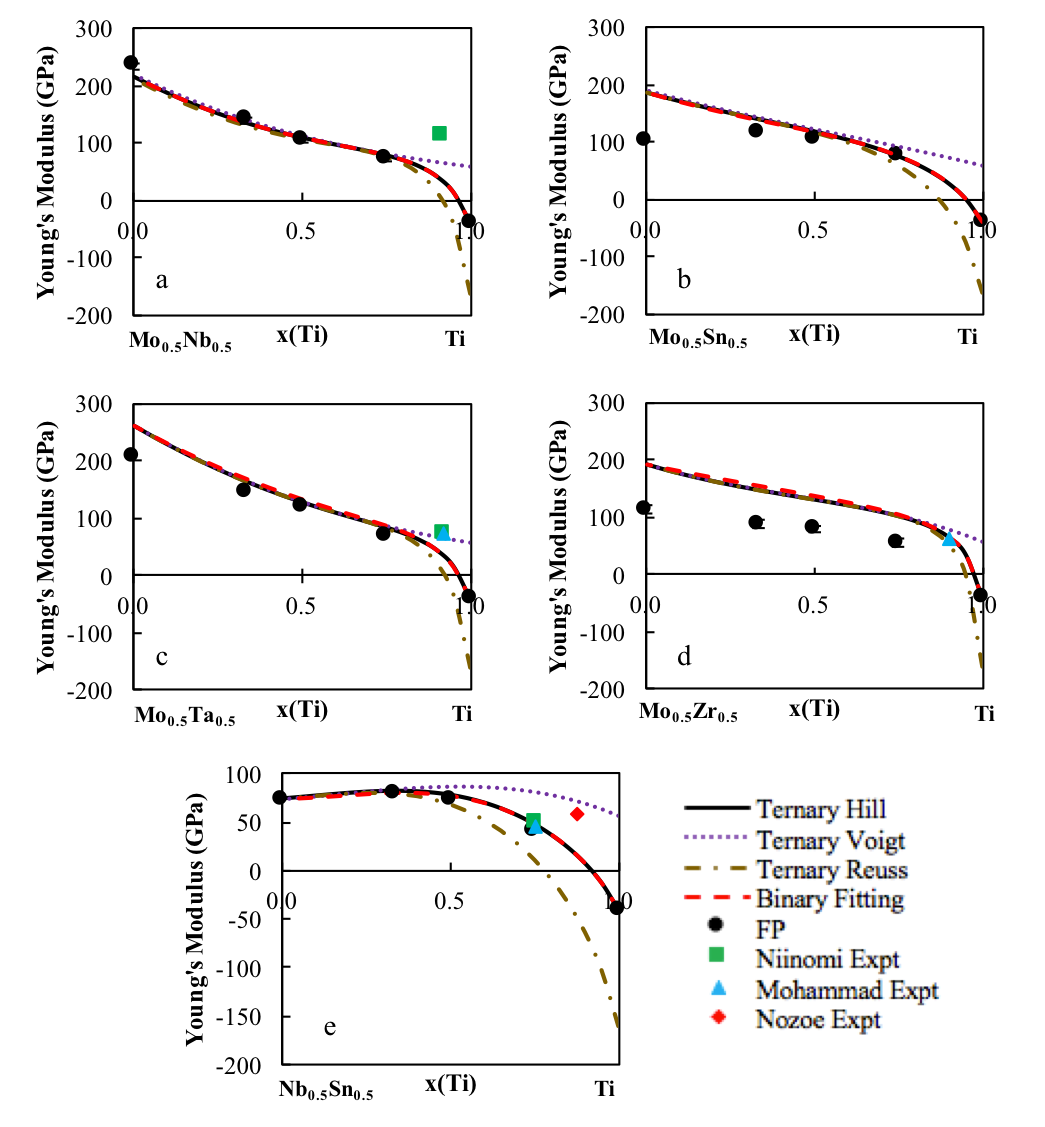
\includegraphics[width=\textwidth]{Chapter-6/Figures/tixyyoungs1.png}
	\caption{Young's modulus \textit{E} of five of the Ti-X-Y ternary systems are plotted from a 50-50 mixture of the alloying elements to Ti in the bcc phase. The present calculations are plotted as filled circles with the error bars. The red dotted line is the extrapolation for the pure elements and binary interaction parameters only. The dotted purple line is the Voigt upper Young’s modulus bound, the gold dot dashed line is the lower Reuss Young’s modulus bound and the black line is the Hill Young’s modulus average. Experimental values are include for comparison \cite{Niinomi2012,Mohammed2014,Nozoe2007,Geetha2009}.}
	\label{Ch6-figure:tixyyoungs1}
\end{figure}

\pagebreak
\begin{figure}[H]
	\centering
	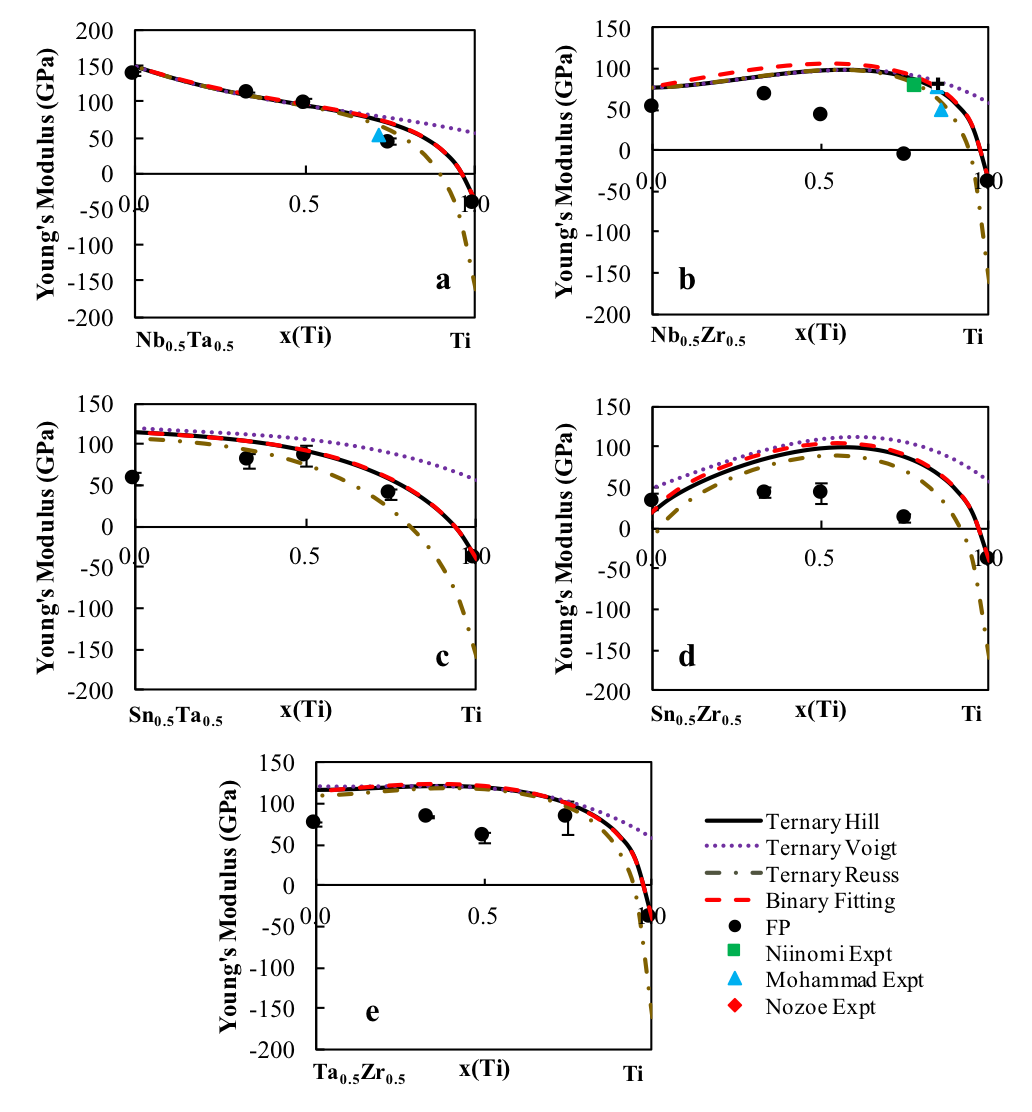
\includegraphics[width=\textwidth]{Chapter-6/Figures/tixyyoungs2.png}
	\caption{Young's modulus \textit{E} of five of the Ti-X-Y ternary systems are plotted from a 50-50 mixture of the alloying elements to Ti in the bcc phase. The present calculations are plotted as filled circles with the error bars. The red dotted line is the extrapolation for the pure elements and binary interaction parameters only. The dotted purple line is the Voigt upper Young’s modulus bound, the gold dot dashed line is the lower Reuss Young’s modulus bound and the black line is the Hill Young’s modulus average. Experimental values are include for comparison \cite{Niinomi2012,Mohammed2014,Nozoe2007,Geetha2009}.}
	\label{Ch6-figure:tixyyoungs2}
\end{figure}

\pagebreak
\begin{figure}[H]
	\centering
	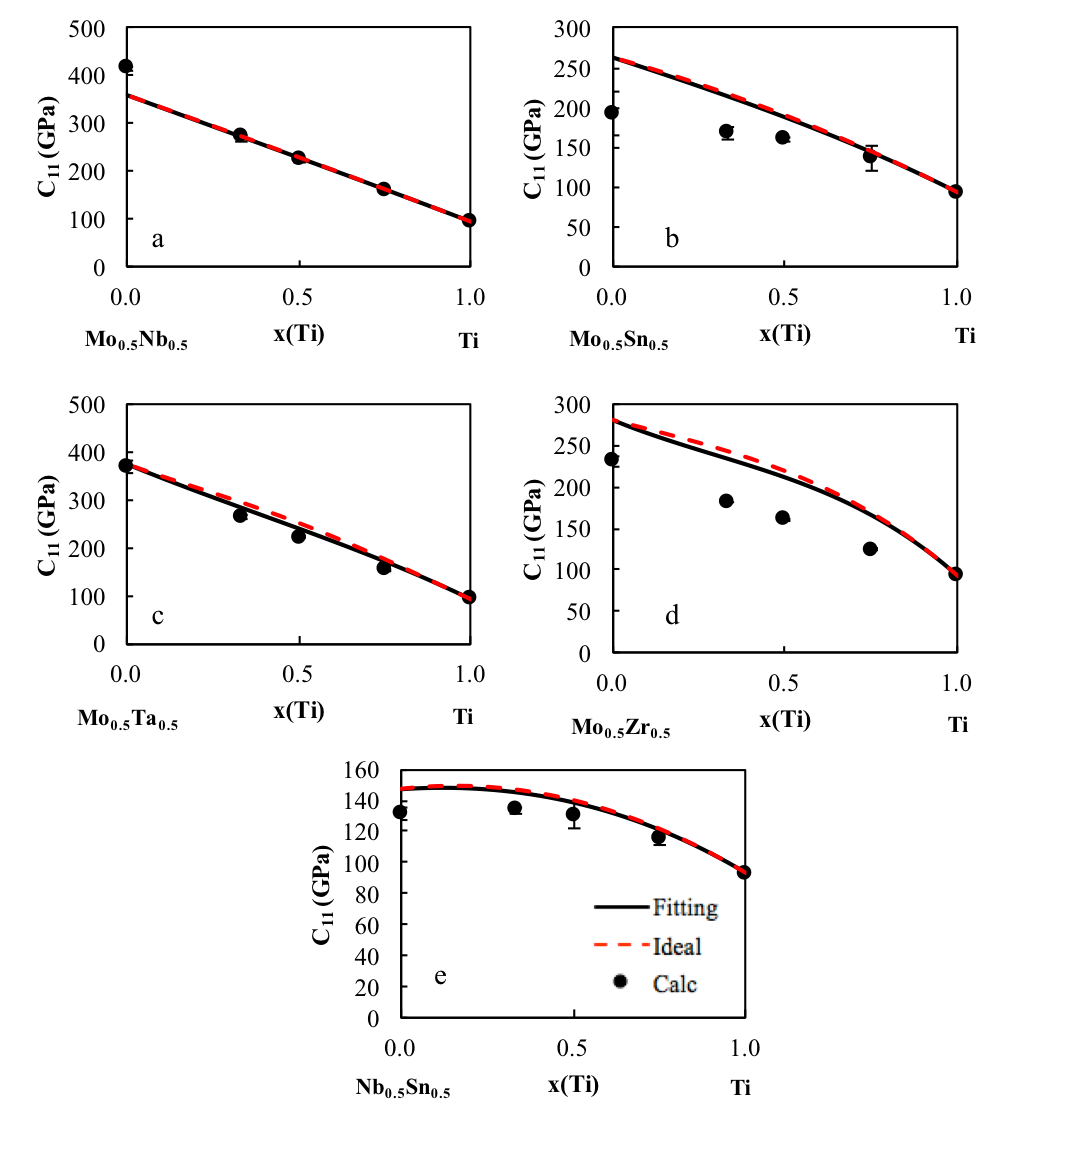
\includegraphics[width=\textwidth]{Chapter-6/Figures/tixyc11_1.png}
	\caption{Calculated $\overline{C}_{11}$ values (circles) plotted with their errors as well as the interpolation from the binary interaction parameters (red dashed line) and the ternary fitting (black dashed line) for five of the Ti-X-Y binary systems from a 50-50 mixture of the alloying elements X and Y to Ti (X$\neq$Y=Mo, Nb, Ta, Sn, Zr).}
	\label{Ch6-figure:tixyc11_1}
\end{figure}

\pagebreak
\begin{figure}[H]
	\centering
	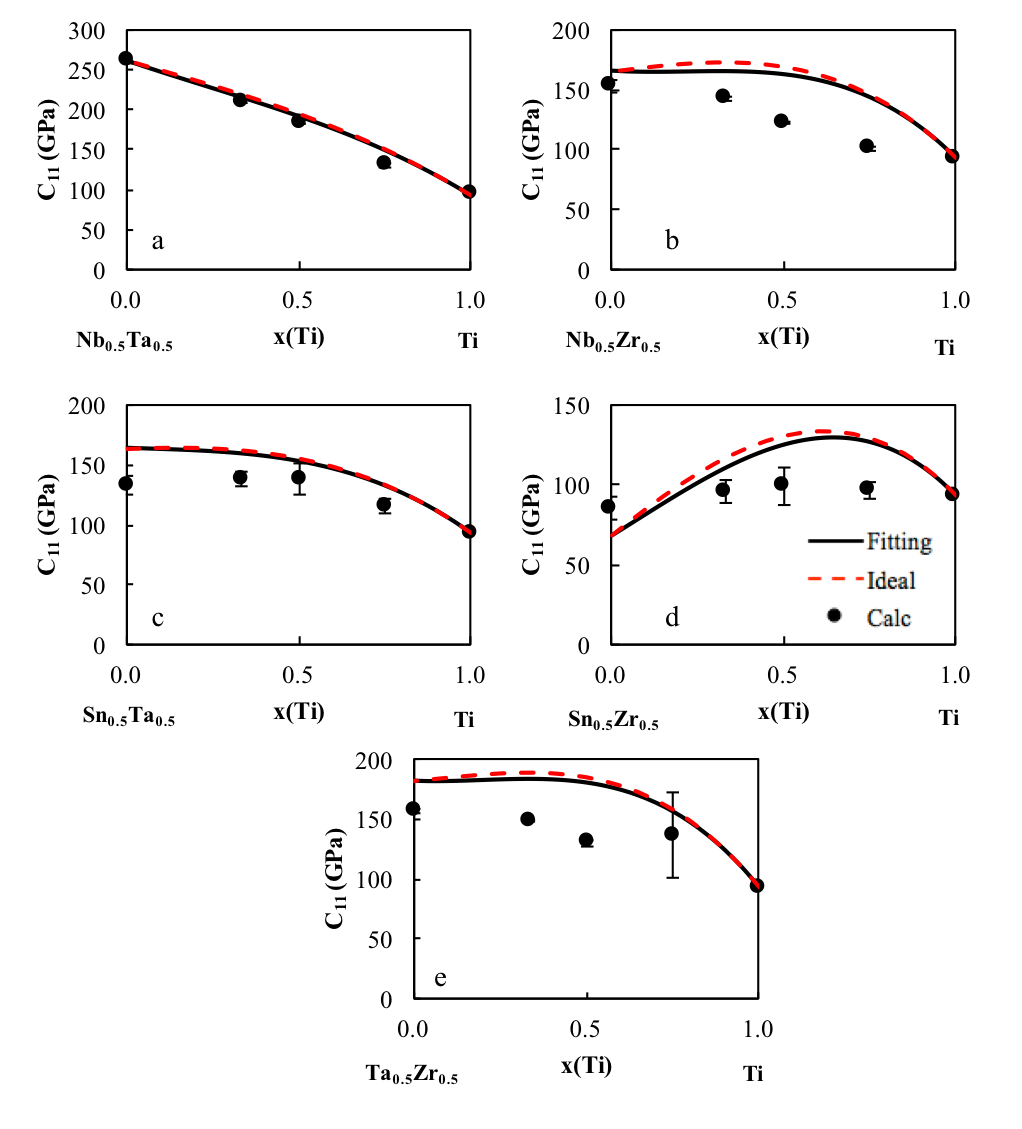
\includegraphics[width=\textwidth]{Chapter-6/Figures/tixyc11_2.png}
	\caption{Calculated $\overline{C}_{11}$ values (circles) plotted with their errors as well as the interpolation from the binary interaction parameters (red dashed line) and the ternary fitting (black dashed line) for five of the Ti-X-Y binary systems from a 50-50 mixture of the alloying elements X and Y to Ti (X$\neq$Y=Mo, Nb, Ta, Sn, Zr).}
	\label{Ch6-figure:tixyc11_2}
\end{figure}

\pagebreak
\begin{figure}[H]
	\centering
	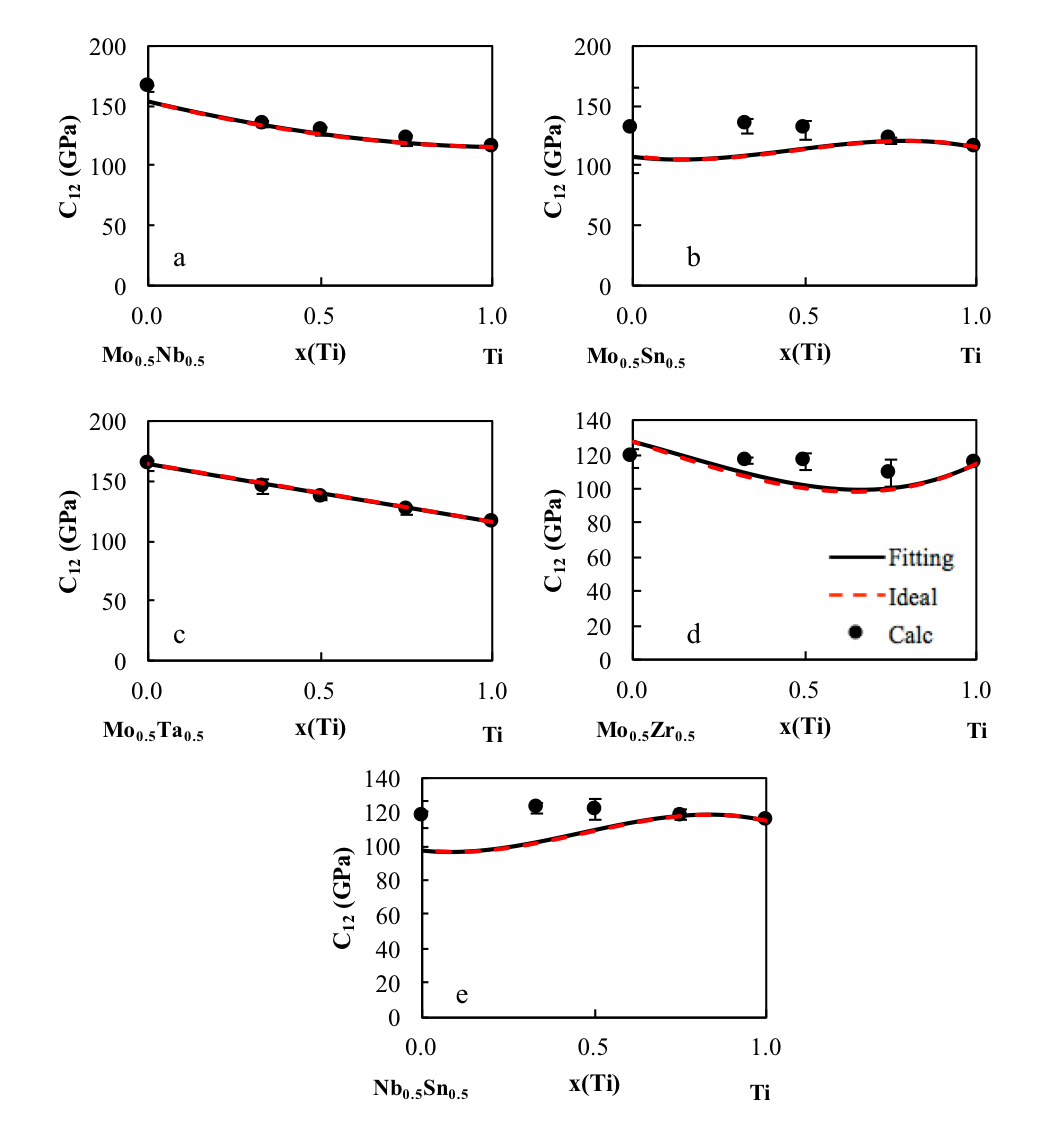
\includegraphics[width=\textwidth]{Chapter-6/Figures/tixyc12_1.png}
	\caption{Calculated $\overline{C}_{12}$ values (circles) plotted with their errors as well as the interpolation from the binary interaction parameters (red dashed line) and the ternary fitting (black dashed line) for five of the Ti-X-Y binary systems from a 50-50 mixture of the alloying elements X and Y to Ti (X$\neq$Y=Mo, Nb, Ta, Sn, Zr).}
	\label{Ch6-figure:tixyc12_1}
\end{figure}

\pagebreak
\begin{figure}[H]
	\centering
	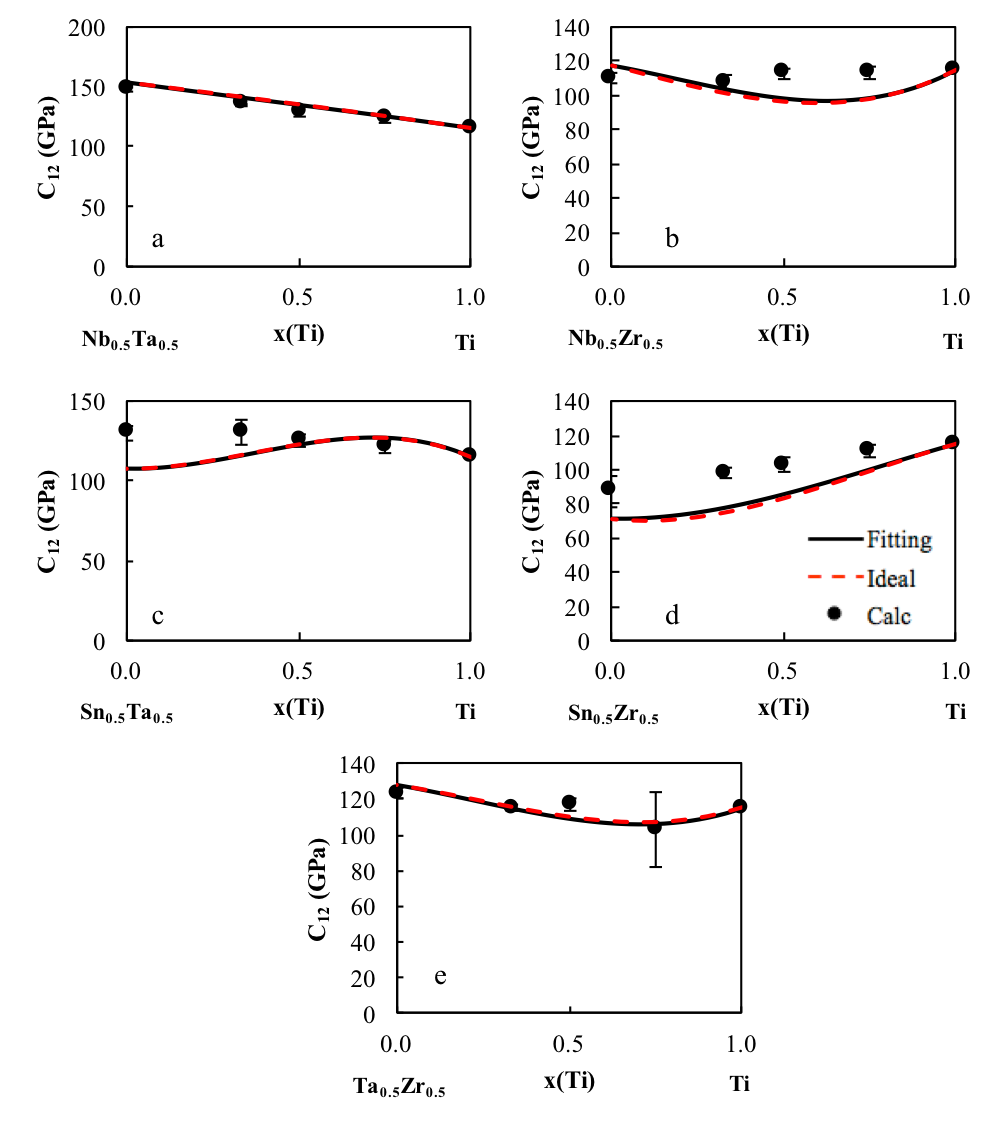
\includegraphics[width=\textwidth]{Chapter-6/Figures/tixyc12_2.png}
	\caption{Calculated $\overline{C}_{12}$ values (circles) plotted with their errors as well as the interpolation from the binary interaction parameters (red dashed line) and the ternary fitting (black dashed line) for five of the Ti-X-Y binary systems from a 50-50 mixture of the alloying elements X and Y to Ti (X$\neq$Y=Mo, Nb, Ta, Sn, Zr).}
	\label{Ch6-figure:tixyc12_2}
\end{figure}

\pagebreak
\begin{figure}[H]
	\centering
	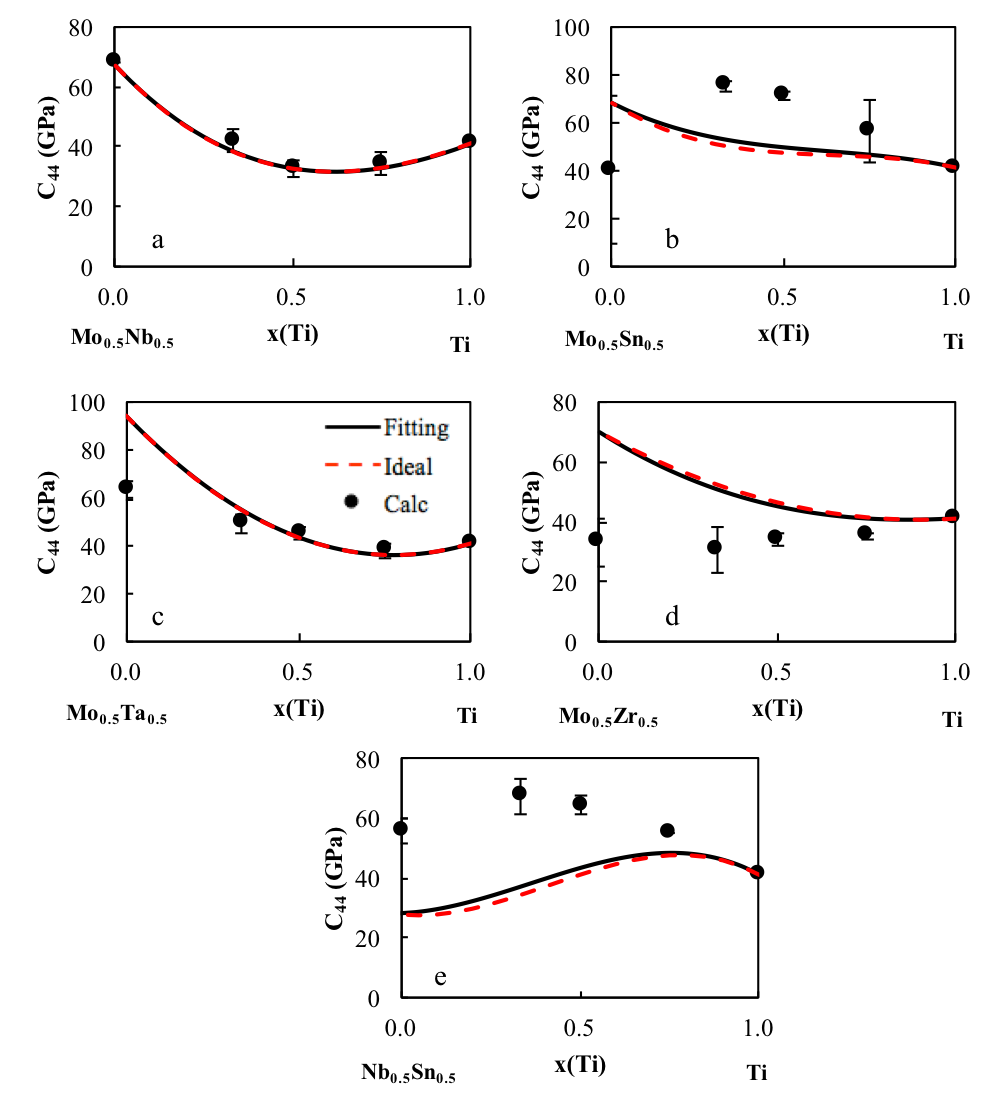
\includegraphics[width=\textwidth]{Chapter-6/Figures/tixyc44_1.png}
	\caption{Calculated $\overline{C}_{44}$ values (circles) plotted with their errors as well as the interpolation from the binary interaction parameters (red dashed line) and the ternary fitting (black dashed line) for five of the Ti-X-Y binary systems from a 50-50 mixture of the alloying elements X and Y to Ti (X$\neq$Y=Mo, Nb, Ta, Sn, Zr).}
	\label{Ch6-figure:tixyc44_1}
\end{figure}

\pagebreak
\begin{figure}[H]
	\centering
	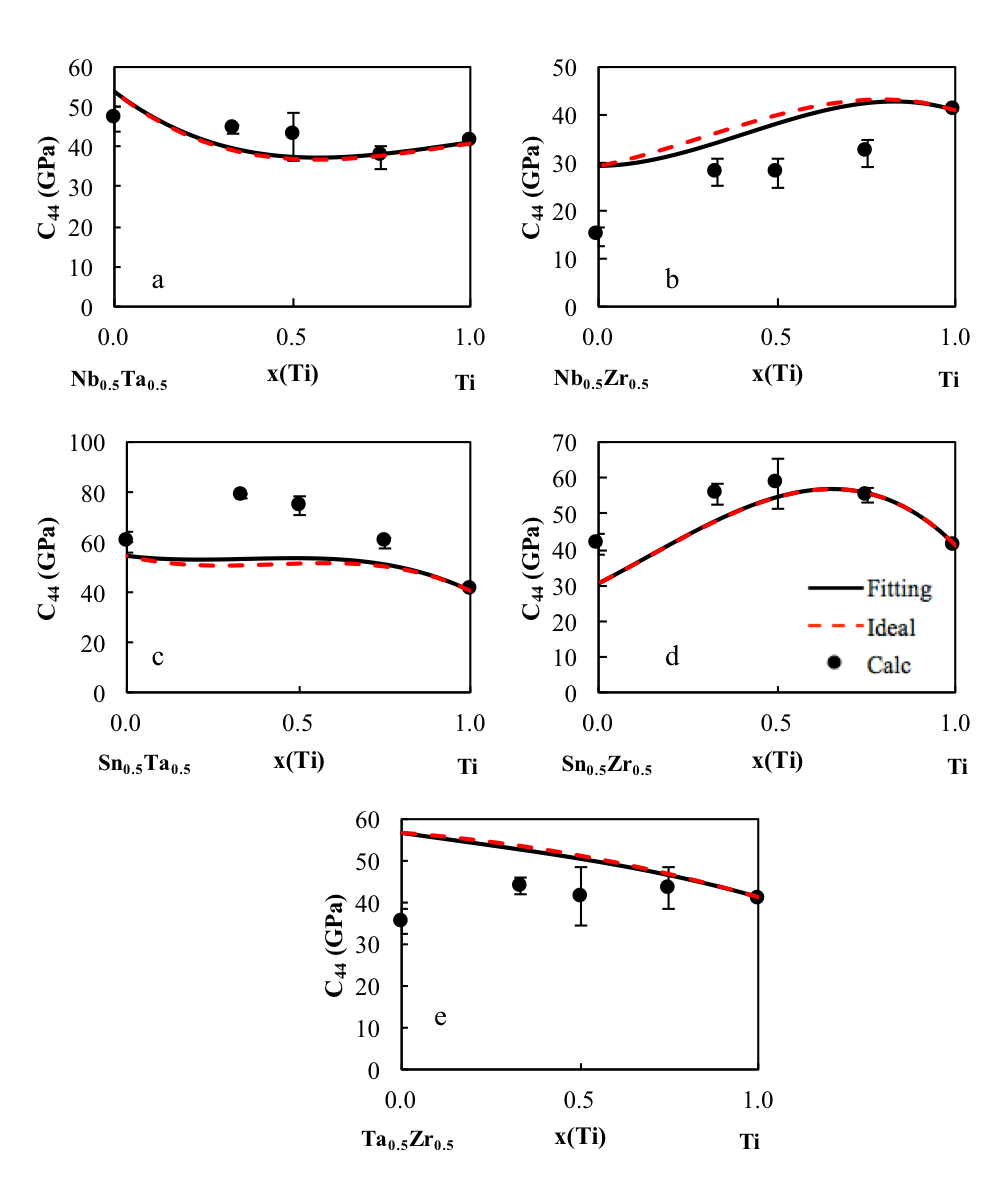
\includegraphics[width=\textwidth]{Chapter-6/Figures/tixyc44_2.png}
	\caption{Calculated $\overline{C}_{44}$ values (circles) plotted with their errors as well as the interpolation from the binary interaction parameters (red dashed line) and the ternary fitting (black dashed line) for five of the Ti-X-Y binary systems from a 50-50 mixture of the alloying elements X and Y to Ti (X$\neq$Y=Mo, Nb, Ta, Sn, Zr).}
	\label{Ch6-figure:tixyc44_2}
\end{figure}

\pagebreak
\begin{figure}[H]
	\centering
	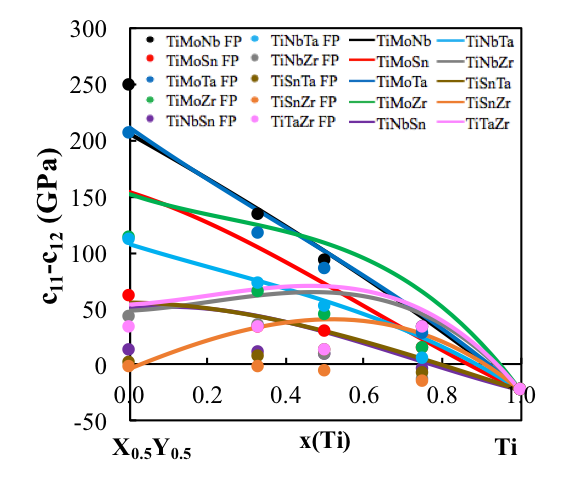
\includegraphics[width=\textwidth]{Chapter-6/Figures/tixyc11-c12.png}
	\caption{Calculated $\overline{C}_{11}$-$\overline{C}_{12}$ values (circles) plotted with the present modeling (solid lines) for the Ti-X-Y ternary systems (X$\neq$Y=Mo, Nb, Ta, Sn, Zr). The $\overline{C}_{11}$-$\overline{C}_{12}$ shows the stability of the bcc phase, when the value is negative the bcc phase is not stable in the corresponding composition ranges.}
	\label{Ch6-figure:tixyc11-c12}
\end{figure}

\pagebreak
\begin{figure}[H]
	\centering
	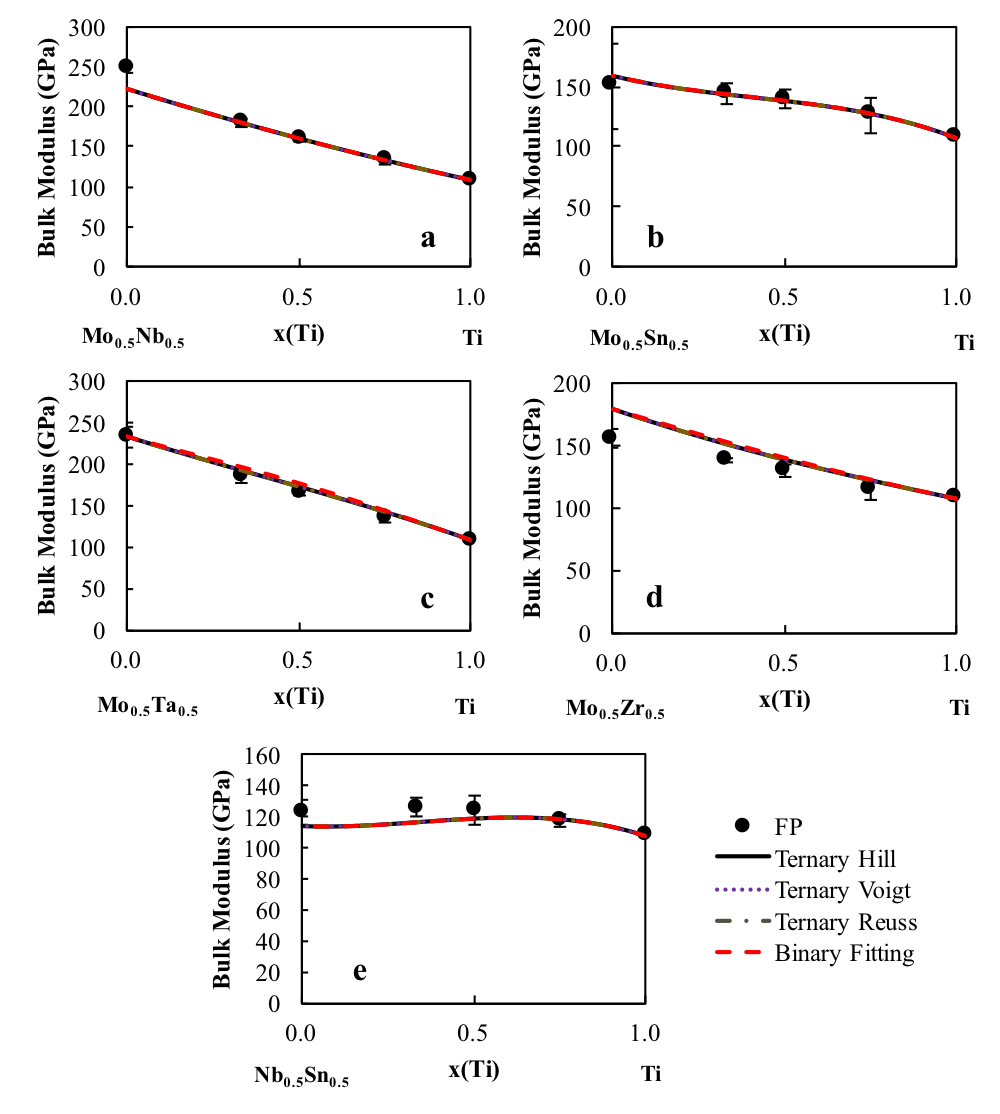
\includegraphics[width=\textwidth]{Chapter-6/Figures/tixybulk1.png}
	\caption{Bulk modulus \textit{B} calculations of five of the Ti-X-Y ternary systems (X$\neq$Y=Mo, Nb, Ta, Sn, Zr). The present calculations are plotted as the filled circles with error bars as well as the interpolation from the binary interaction parameters (red dashed line). The dotted purple line is the Voigt upper bulk modulus bound, the gold dashed line is the lower Reuss bulk modulus bound and the black line is the Hill bulk modulus average plotted from a 50-50 mixture of the alloying elements X and Y to Ti.}
	\label{Ch6-figure:tixybulk1}
\end{figure}

\pagebreak
\begin{figure}[H]
	\centering
	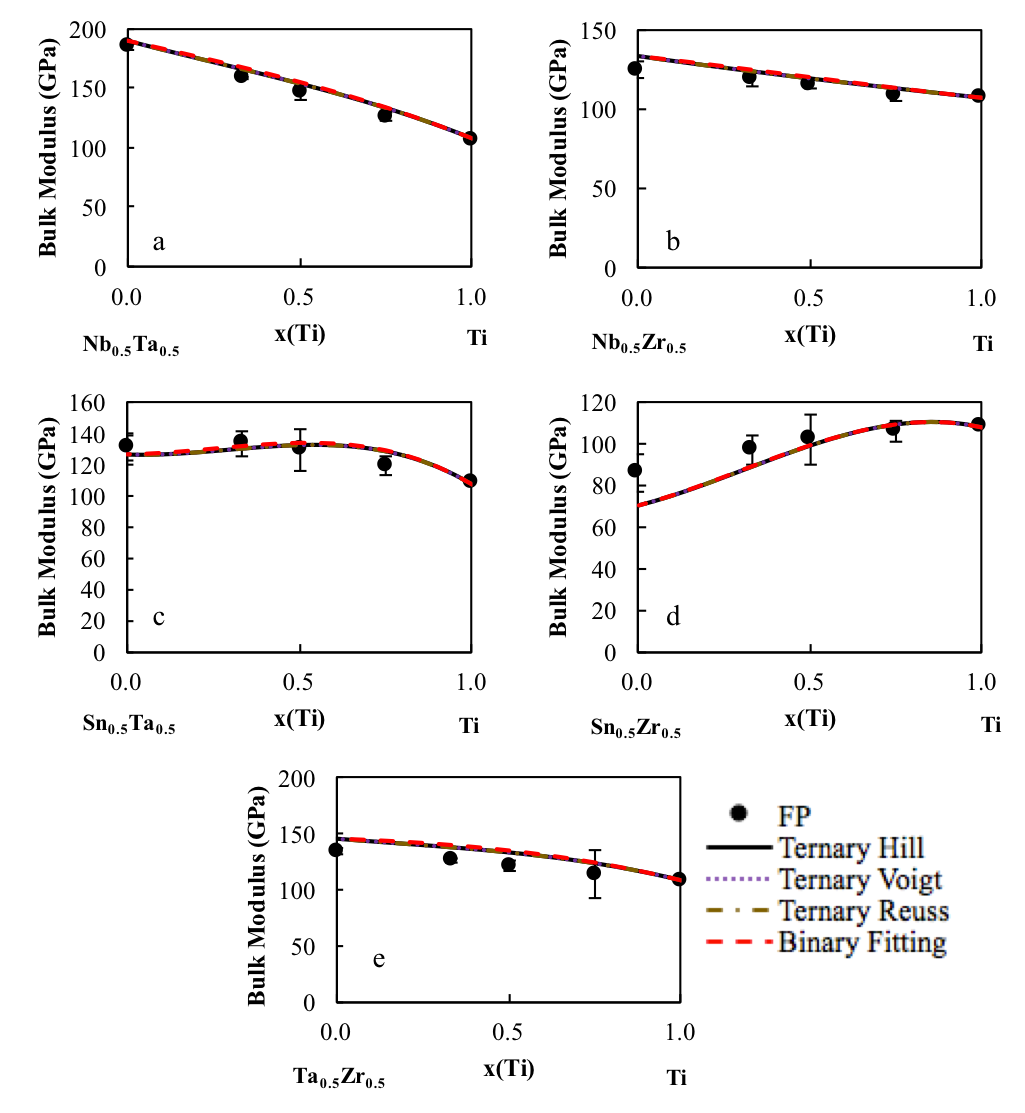
\includegraphics[width=\textwidth]{Chapter-6/Figures/tixybulk2.png}
	\caption{Bulk modulus \textit{B} calculations of five of the Ti-X-Y ternary systems (X$\neq$Y=Mo, Nb, Ta, Sn, Zr). The present calculations are plotted as the filled circles with error bars as well as the interpolation from the binary interaction parameters (red dashed line). The dotted purple line is the Voigt upper bulk modulus bound, the gold dashed line is the lower Reuss bulk modulus bound and the black line is the Hill bulk modulus average plotted from a 50-50 mixture of the alloying elements X and Y to Ti.}
	\label{Ch6-figure:tixybulk2}
\end{figure}

\pagebreak
\begin{figure}[H]
	\centering
	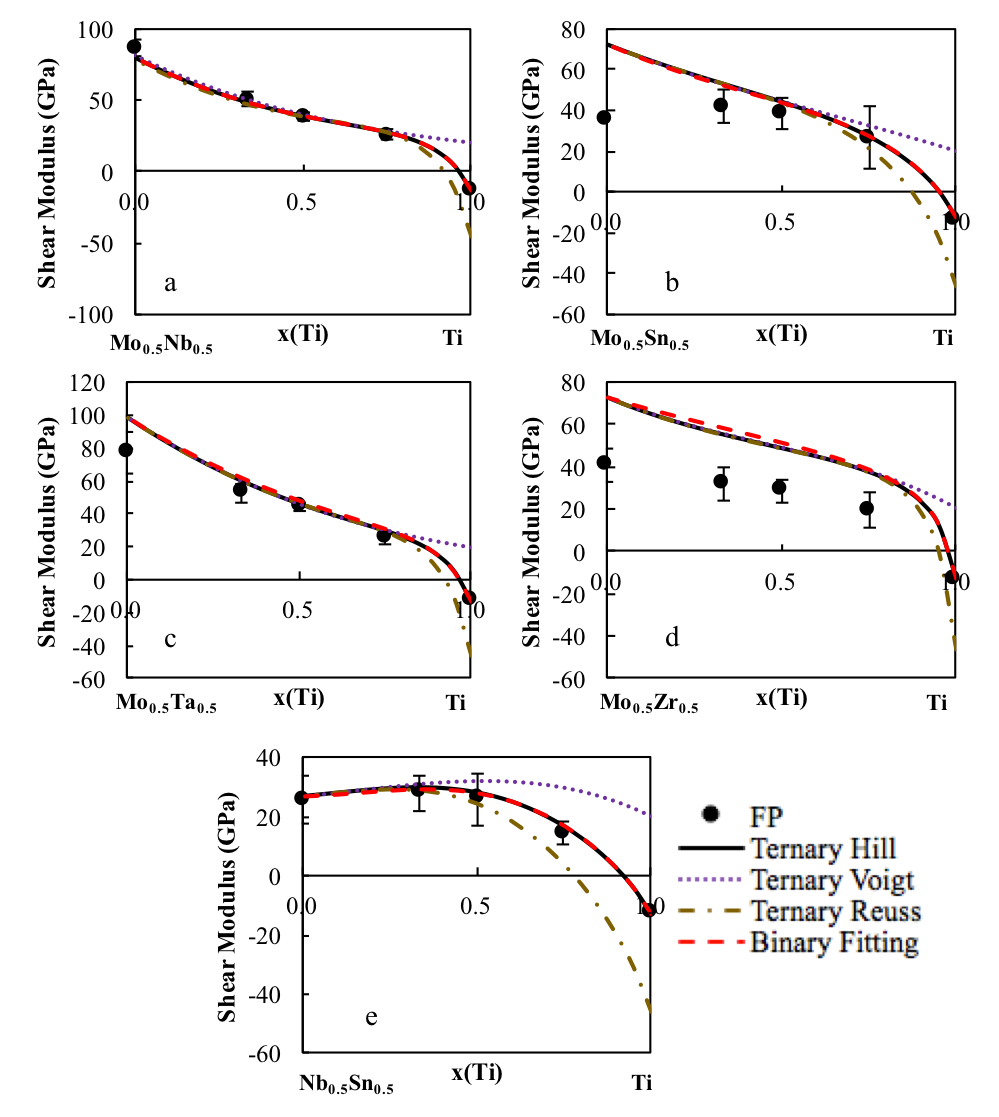
\includegraphics[width=\textwidth]{Chapter-6/Figures/tixyshear1.png}
	\caption{Shear modulus \textit{G} calculations of five of the Ti-X-Y ternary systems (X$\neq$Y=Mo, Nb, Ta, Sn, Zr). The present calculations are plotted as the filled circles with error bars as well as the interpolation from the binary interaction parameters (red dashed line). The dotted purple line is the Voigt upper shear modulus bound, the gold dashed line is the lower Reuss shear modulus bound and the black line is the Hill shear modulus average plotted from a 50-50 mixture of the alloying elements X and Y to Ti.}
	\label{Ch6-figure:tixyshear1}
\end{figure}

\pagebreak
\begin{figure}[H]
	\centering
	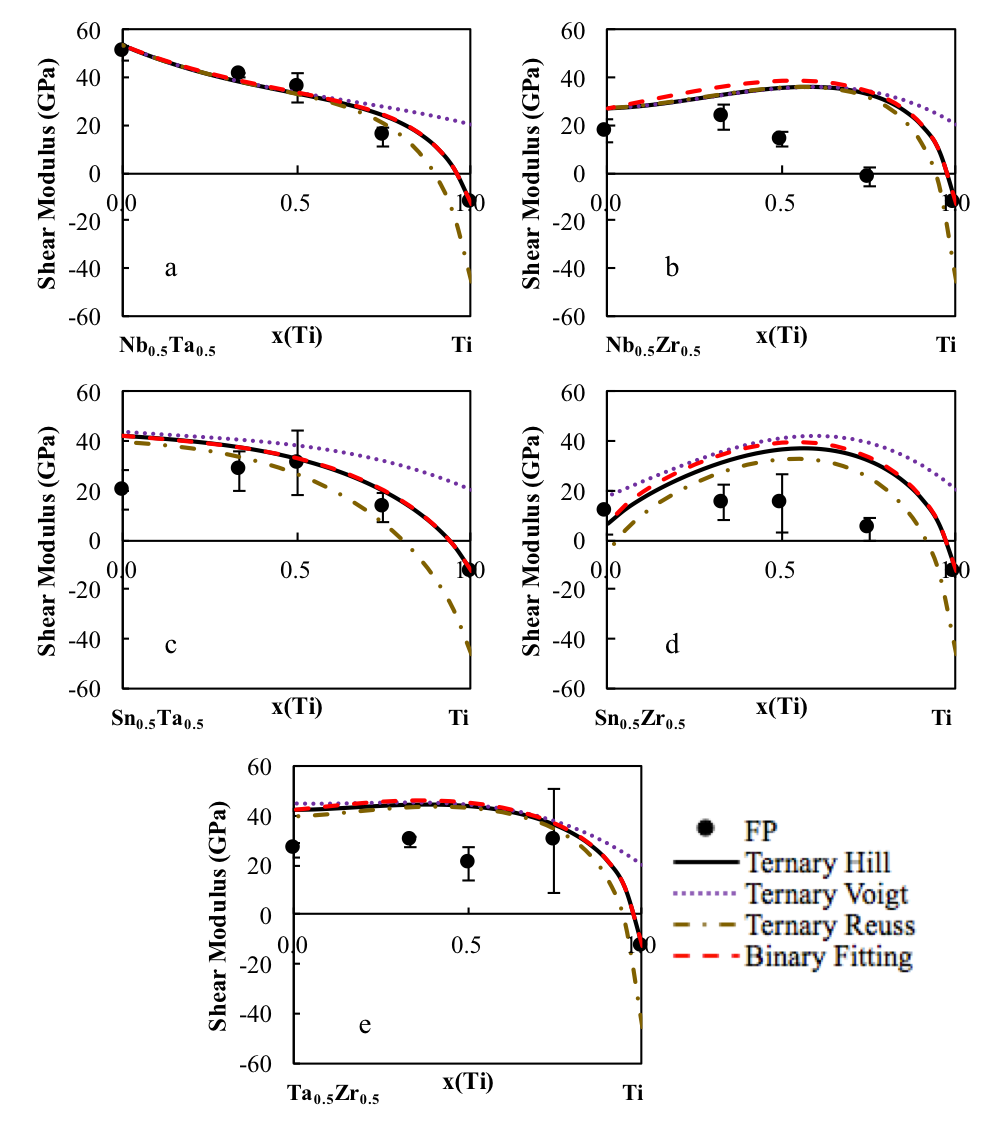
\includegraphics[width=\textwidth]{Chapter-6/Figures/tixyshear2.png}
	\caption{Shear modulus \textit{G} calculations of five of the Ti-X-Y ternary systems (X$\neq$Y=Mo, Nb, Ta, Sn, Zr). The present calculations are plotted as the filled circles with error bars as well as the interpolation from the binary interaction parameters (red dashed line). The dotted purple line is the Voigt upper shear modulus bound, the gold dashed line is the lower Reuss shear modulus bound and the black line is the Hill shear modulus average plotted from a 50-50 mixture of the alloying elements X and Y to Ti.}
	\label{Ch6-figure:tixyshear2}
\end{figure}

\pagebreak
\begin{figure}[H]
	\centering
	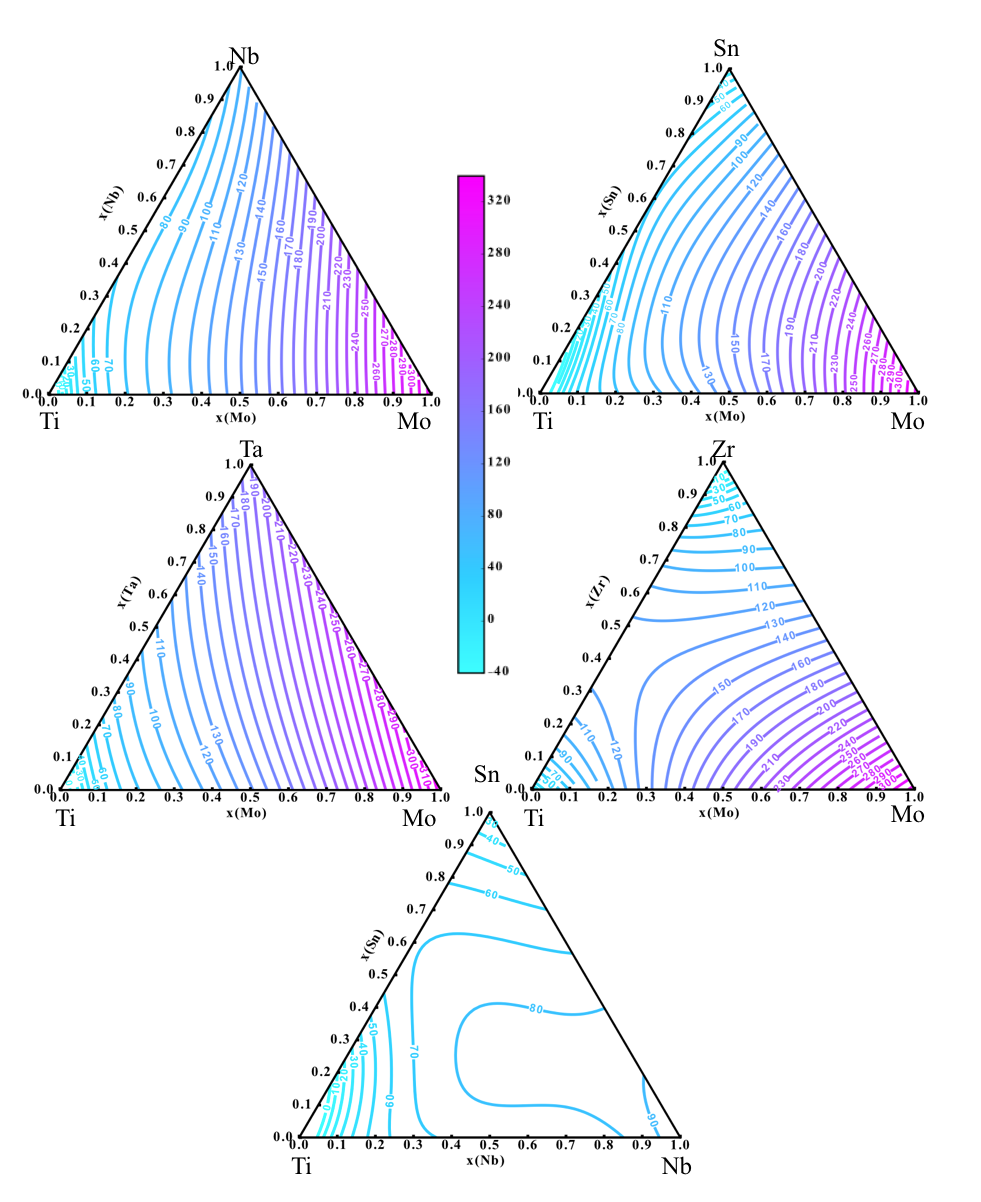
\includegraphics[width=\textwidth]{Chapter-6/Figures/tixymap1.png}
	\caption{The Young's modulus is mapped as a function of composition in GPa for the Ti-Mo-Nb, Ti-Mo-Sn, Ti-Mo-Ta, Ti-Mo-Zr and Ti-Nb-Sn alloy systems using pycalphad \cite{Otis2017}.}
	\label{Ch6-figure:tixymap1}
\end{figure}

\pagebreak
\begin{figure}[H]
	\centering
	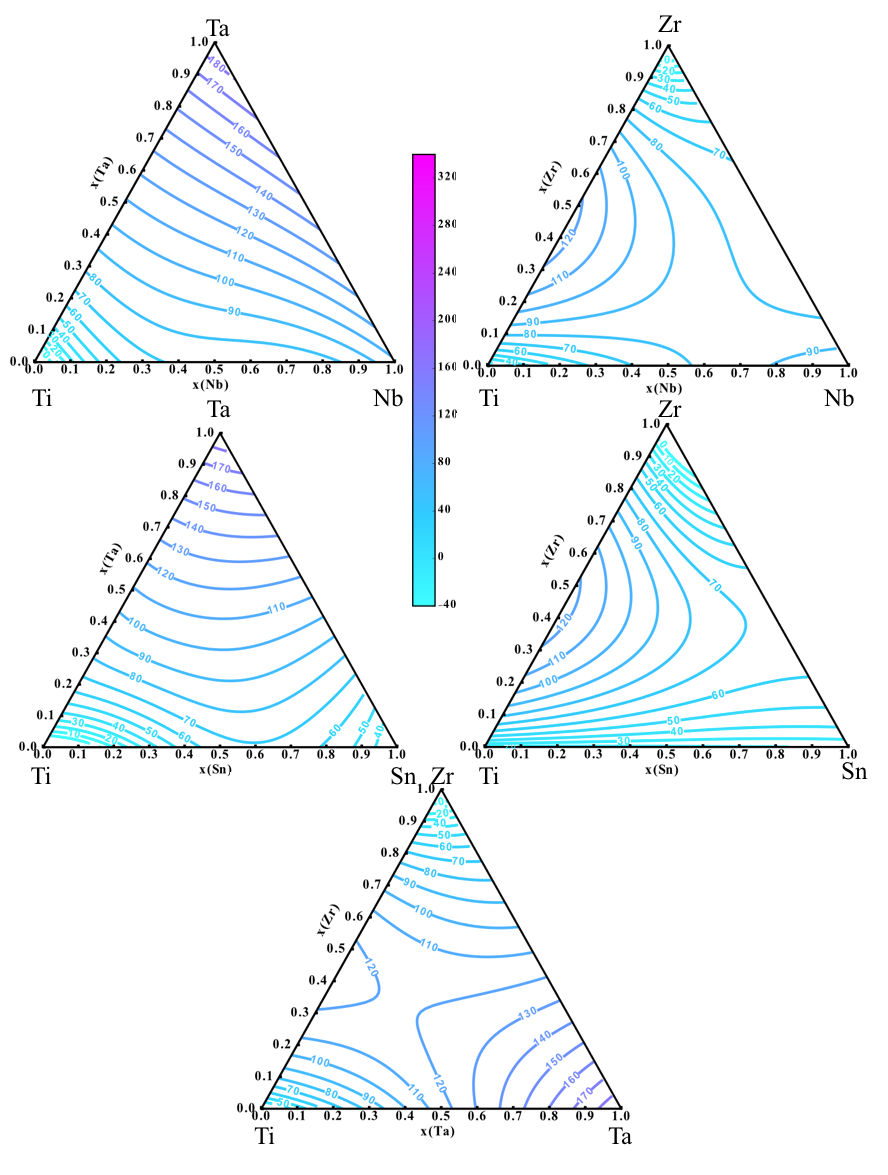
\includegraphics[width=\textwidth]{Chapter-6/Figures/tixymap2.png}
	\caption{The Young's modulus is mapped as a function of composition in GPa for the Ti-Mo-Nb, Ti-Mo-Sn, Ti-Mo-Ta, Ti-Mo-Zr and Ti-Nb-Sn alloy systems using pycalphad \cite{Otis2017}.}
	\label{Ch6-figure:tixymap2}
\end{figure}

\pagebreak
\begin{figure}[H]
	\centering
	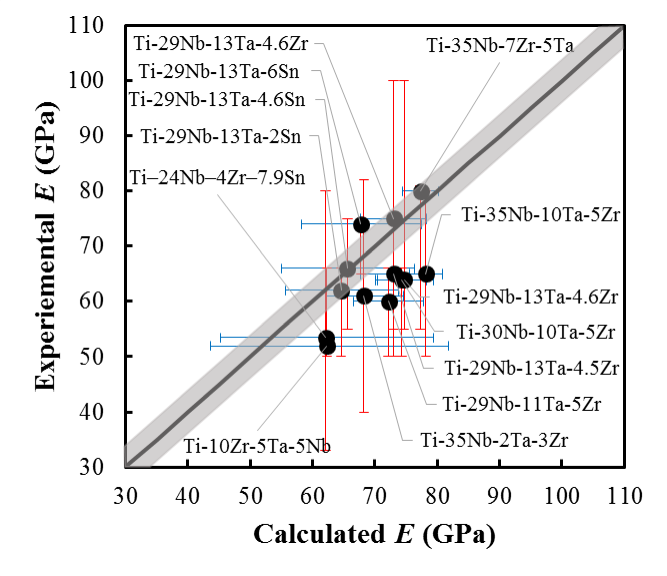
\includegraphics[width=\textwidth]{Chapter-6/Figures/tixydatabase.png}
	\caption{\textit{E} of multicomponent bcc Ti alloys predicted from the completed database are compared with measured experimental results. Error bars plotted are from the variation in experimentally determined Young’s modulus values for the specific multi-component alloy. The grey region refers to the error in the first-principles calculations. More information on the alloys is Table \ref{Ch6-table:tixydatacomp} \cite{Mohammed2014,Geetha2009,Tane2010a}.}
	\label{Ch6-figure:tixydatabase}
\end{figure}